The proposed fixity storage is evaluated on a local installation of the Ethereum blockchain and on the online Ropsten test network, where ETH used for transactions are free of charge.
The two key parameters for evaluation are the operation cost and operation throughput. 
\textit{Operation cost} is calculated by multiplying the number of relevant cost transactions with the average gas cost of a writing transaction on the blockchain, see Eq. \ref{eq:expected_cost}
\begin{equation}\label{eq:expected_cost}
    C = J * Tx_c = \lceil N/k \rceil * (G_{transaction} + G_{txdatanonzero}*Tx_{bytesize})
\end{equation}
where \textit{J} is the number of pools on ingest; \textit{$Tx_c$} is the cost for a transaction in gas, see Section \ref{sec:costs} for the gas cost of certain operations.
I intent to present the operation cost in the form of gas, the unit that measures the amount of computation effort requried to execute specific operations, instead of the cost in USD or EUR. This is because, the amount of gas used during the experiment should stay constant, whereas the price of the ETH token fluctuates heavily. Therefore the amount of gas is a better indicator on how costly the fixity storage is.
\textit{Operation throughput} is measured by operations needed per object utilizing pooled testing compared with the individual testing strategy, where the efficiency of pooling strategy S is expressed by Equation \ref{eq:efficiency}
\begin{equation}\label{eq:efficiency}
    E(S) = N/T(S)
\end{equation}
where, assuming the preservation process of n digital objects without pooling requires N operations and the preservation of the same objects using strategy S requires T(S) operations. In the case of indivudual testing the efficiency of E(N) is 1, whereas if strategy S requires two times less operations the efficiency E(S) is 2 \cite[4]{vzilinskas2021pooled}.

\textit{What is the optimal pool size based on the corruption rates of digital objects in the archive regarding cost and operation throughput?}

Corruption rate $p$ represents the prevalence of corruption, e.g., when I assume that 2000 of 10000 objects will be corrupted during the preservation process, $p = 2000/10000 = 0.2$. 

\textit{Expected Operation Cost:} The optimal pool size, which will result in the lowest number of cost relevant transactions is the number of pools $J$, as seen in eq. \ref{fig:expected_cost}, because I only must write onto the blockchain during the ingest process where the root hashes of pools are persisted.
After the first Iteration of the experiment, the number of corrupt objects per positive pools were included in the first draft of Equation \ref{eq:expected_cost}, where I assumed that I had to re-calculate corrupt pool hashes and re-store them on the blockchain, but these "repairing" actions can be done locally through data scrubbing. I only need to know that the pool is corrupt, then I can to substitute each object in the pool with a correct copy in the archive. For this part of the research question, local operations are out of scope because they do not cause direct cost on the blockchain, therefore the optimal poolsize calculated by Eq. \ref{eq:expected_cost} is $N$, see Figure \ref{fig:expected_cost}. A poolsize of $N$ results in exactly 1 cost relevant transaction since I have combined every object on ingest into a hash-list which's root will be stored on the blockchain. This solution does not scale well, e.g., picture the process of retrieving a single object from the archive. In order to guarantee that the object is unaltered, I would have to re-compute the hash list from every object in the archive (or the bulk ingest in question). Additionally, if the single pool is corrupted, I must replace the whole bulk with copies. 
So, there must be an answer, which rewards smaller poolsizes to avoid data scrubbing. Eq. \ref{eq:expected_operations} accounts in the number of times I have to perform data scrubbing in the archive, therefore the data scrubbing actions are included in the operation throughput, since they have to be performed at retrieval in the archive.
\begin{equation}\label{eq:expected_operations}
    T(S) = J + J_+ * k = \lceil N/k \rceil + ((1-(1-p)^k)* \lceil N/k \rceil) * k
\end{equation}
where \textit{J} is the number of pools and \textit{$J_+ * k$} is the number of digital objects in corrupted pools. Therefore the number of expected operations is the number of writing operations on ingest plus the number of data scrubbing operations on retrieval. By adding the amound of data scrubbing operations, the optimal pool size gets significantly lower, see Figure \ref{fig:expected_throughput} The optimal poolsize \text{k} can be determined by finding the minimum of Eq. \ref{eq:expected_operations}, which results in the highest efficiency in Eq. \ref{eq:efficiency}.
\begin{figure}[b]%
    \centering
    \begin{subfigure}{6cm}
    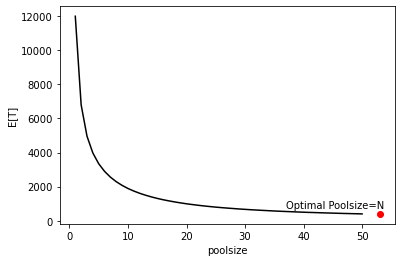
\includegraphics[width=\linewidth]{graphics/expected_cost.png}
    \caption{Expected Cost}\label{fig:expected_cost}
    \end{subfigure}
    \qquad
    \begin{subfigure}{6cm}
    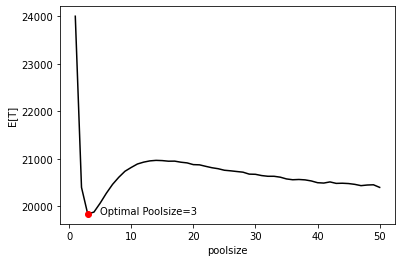
\includegraphics[width=\linewidth]{graphics/expected_throughput.png}
    \caption{Expected Throughput}\label{fig:expected_throughput}
    \end{subfigure}
    \caption{Comparison of optimal poolsizes}%
    \label{fig:optimal_pool_size}%
\end{figure}
In Table \ref{tb:expected costs}  it is shown that for ingest bulks with higher prevalence of corruption rate, smaller poolsizes are favorable.
\begin{table}[h]
    \caption{Expected transaction throughput with different prevalence of corruption rates}
    \centering
    \begin{tabular}{ c c c c}
    \label{tb:expected costs}
     N & p & k & E[T] \\ 
     10000 & 0.01 & 10 & 12052 \\ 
     \hline
     10000 & 0.02 & 8 & 12929 \\  
     \hline
     10000 & 0.1 & 4 & 16799 \\  
     \hline
     10000 & 0.15 & 4 & 18475 \\  
     \hline
     10000 & 0.2 & 3 & 19842  
    \end{tabular}
\end{table}
\textit{To what extend can pooled object hashes increase the transaction throughput and reduce cost for a fixity information storage service on the Ethereum blockchain?}
\label{sec:rq2}
The efficiency of a pooling strategy were measured by savings of tests (in times) using a pooling strategy comparing with the individual testing of a target population. Assuming that the testing of a population of n individuals without pooling requires n tests and the testing of the same population using the strategy S requires T(S) tests, the efficiency of the strategy S can be mathematically expressed by 
\begin{equation}\label{eq:expected_throughput}
    E(S) = N/T(S)
\end{equation}
In the case of individual testing which requires to test all samples, E(S) = 1. If a strategy S requires two times less tests than the individual testing, then E(S) = 2. A larger efciency value means a better efciency of the strategy \cite[4]{vzilinskas2021pooled}.
\subsection{Evenly Distributed corruption rates}
\subsection{Context-Sensitive}
\cite[4]{deckert2020simulation}
\section{RQ 3 Given that metadata has a higher corruption rate, what effect has the split of metadata and objects on the operation cost?}